\chapter{Il percorso di stage }\label{cap:Il_percorso}
\section{Formazione}
Il processo di formazione che mi è stato fornito ha avuto un ruolo fondamentale nella buona riuscita del progetto di stage, 
ha avuto una durata di circa 4 settimane. \\
La causa del protrarsi del processo di formazione è stata provocata dal fatto che concetti legati all'architettura \gls{eda}{},
\textbf{Apache Kafka}, \textbf{Apache Druid}, \textbf{Docker Compose} sono state del tutto innovative per me.\\
Tutto il processo di formazione è stato tracciato e monitorato dal tutor aziendale e da me stesso attraverso le \gls{board}{} offerte 
dal software di project management \textbf{ClickUp} (Figura \ref{cap:ClickUp}).\\
\begin{figure}[h]
    \centering
    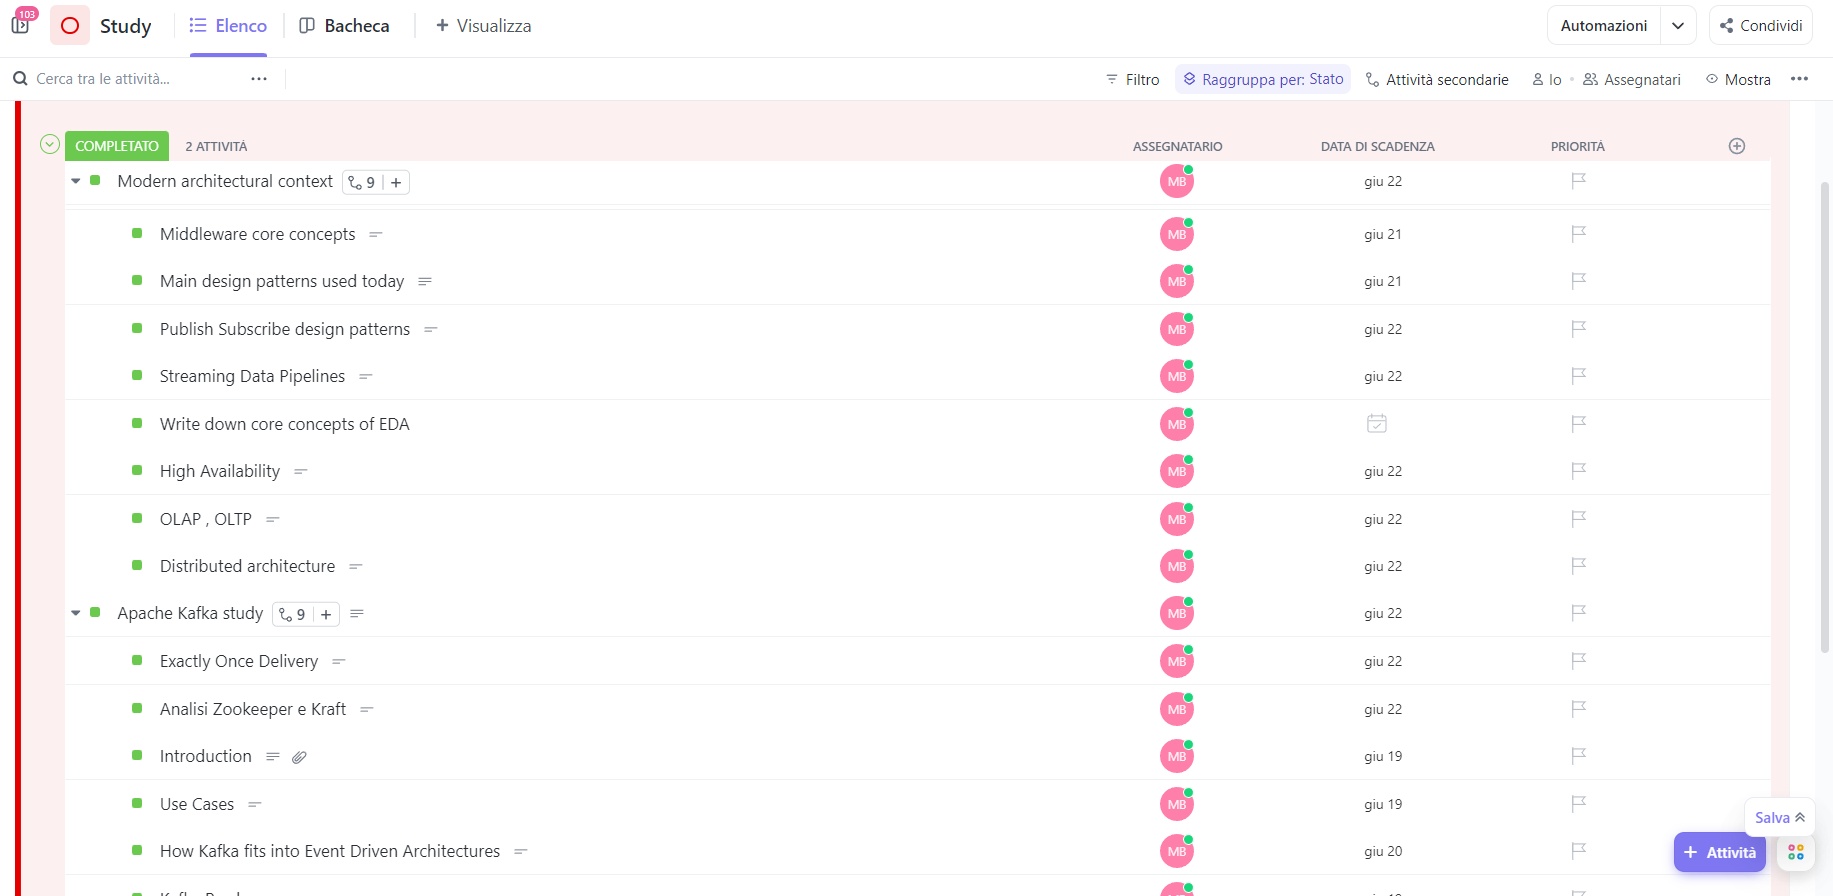
\includegraphics[width=1\textwidth]{images/percorso/formazione.png}
    \caption{Board di ClickUp per il processo di formazione}
    \label{cap:ClickUp}
\end{figure}
\pagebreak
\\
Inoltre durante il processo di formazione, oltre a reperire informazioni da documentazione ufficiale fornita, ho avuto anche modo 
di approfondire quanto appena appreso attraverso delle attività di \gls{hands-on}{} che mi hanno permesso di mettere in pratica quanto appreso (Figura \ref{cap:Hands-on}).
\begin{figure}[h]
    \centering
    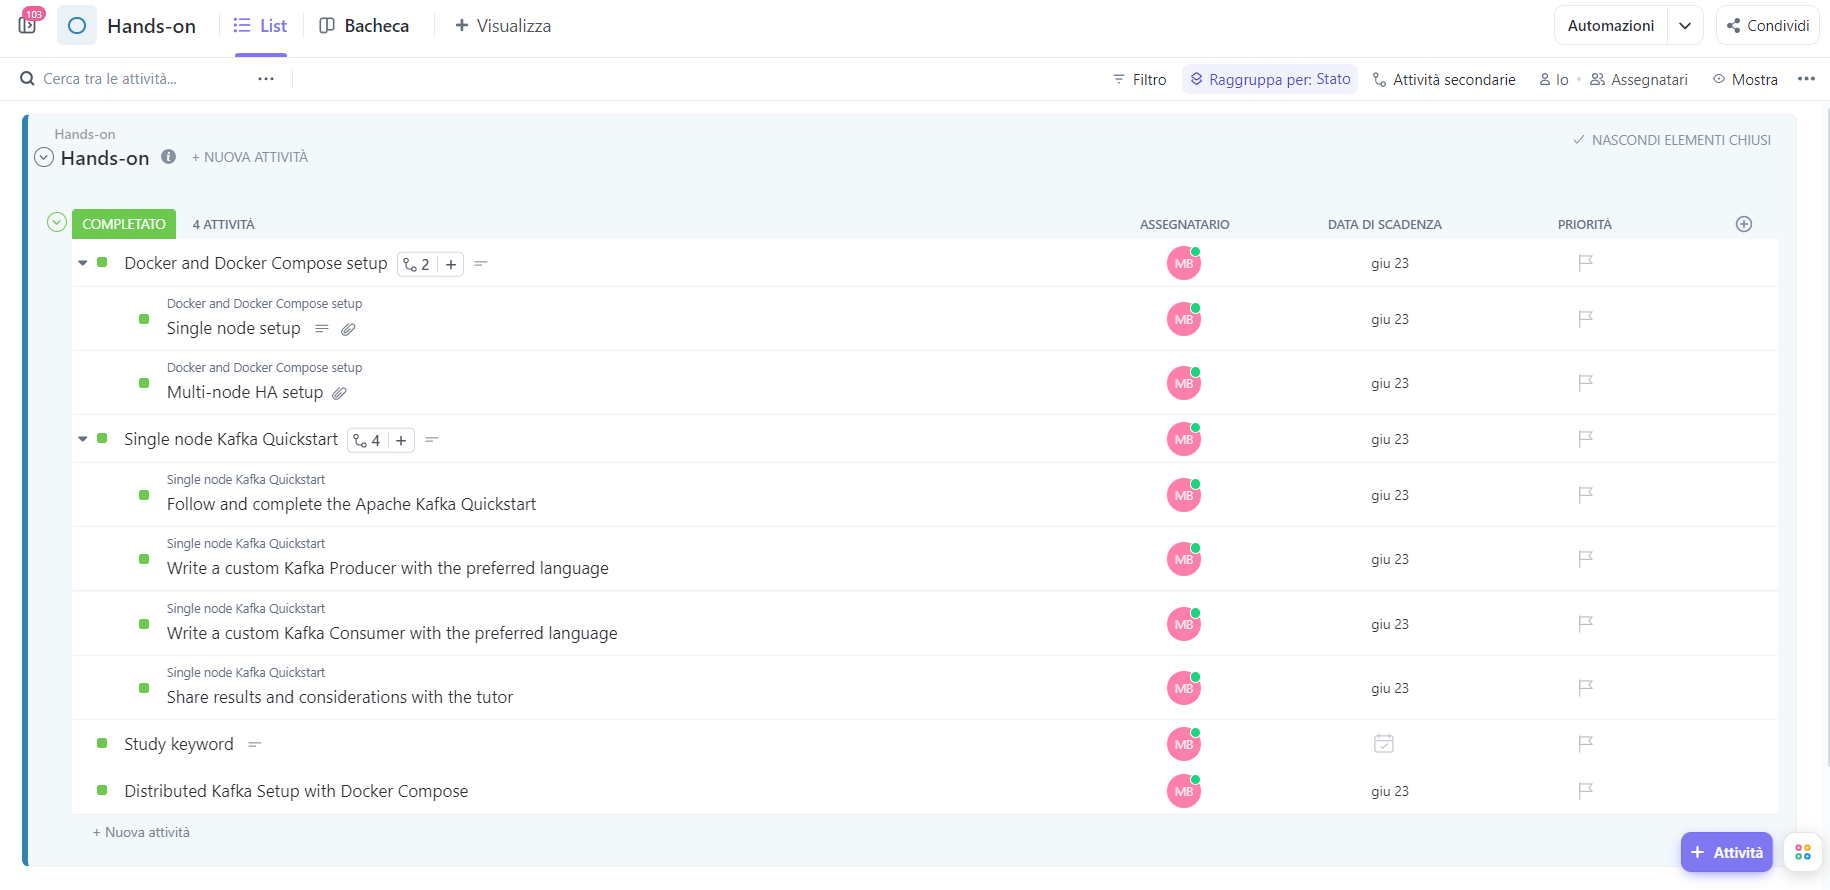
\includegraphics[width=1\textwidth]{images/percorso/hands_on.png}
    \caption{Attività di hands-on per il processo di formazione}
    \label{cap:Hands-on}
\end{figure}
\\
Oltre a ciò, durante il processo di formazione, in collaborazione con il tutor aziendale, è stato definito un processo di coordinamento e produzione di 
documentazione tecnica che mi ha permesso durante tutto lo svolgimento del percorso di stage di avere un tracciamento dei concetti appresi 
e di avere riferimenti per la risoluzione di problemi o dubbi sorti (Figura \ref{cap:Documentazione})
\begin{figure}[h]
    \centering
    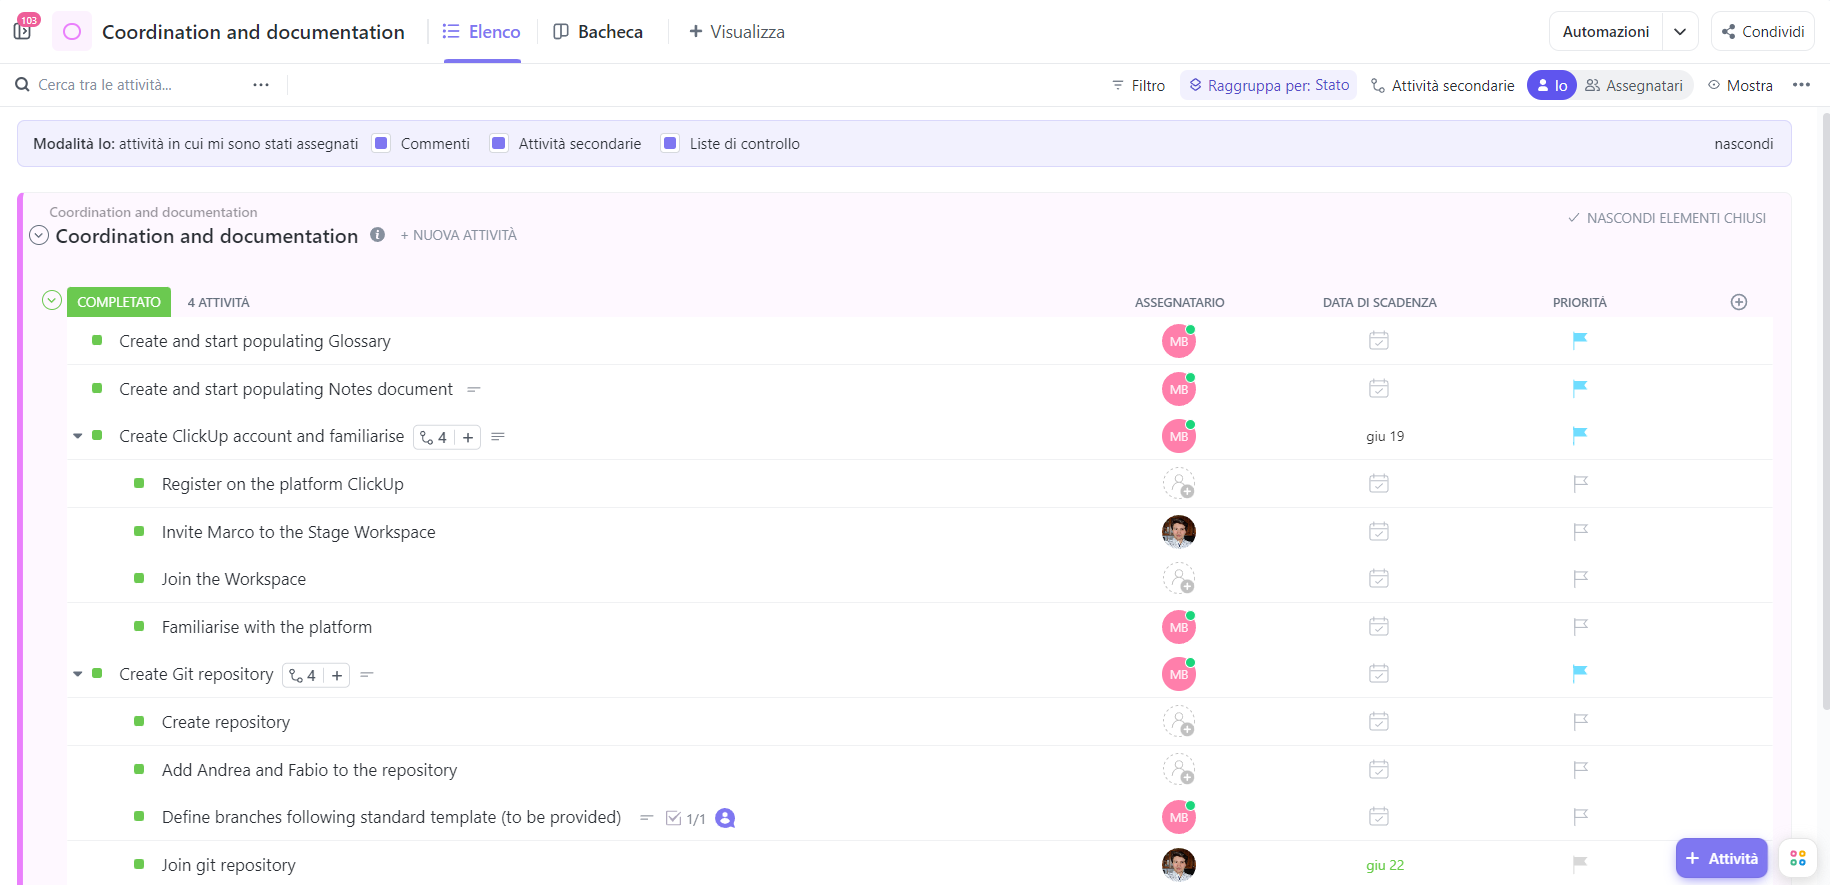
\includegraphics[width=1\textwidth]{images/percorso/coordinamento.png}
    \caption{Board di ClickUp per il processo di coordinamento e documentazione}
    \label{cap:Documentazione}
\end{figure}
\subsection{Daily stand-up meeting}
Durante tutto il percorso di stage, in collaborazione con il tutor aziendale, è stato definito in concomitanza con l'inizio del processo di formazione
è stato definito un processo di \textbf{supporto} ispirato al metodo \gls{Scrum}{}, andando fissare degli incontri giornalieri di circa 15 minuti finalizzati a:
\begin{list}{*}
    \item \textbf{Monitorare} lo stato di avanzamento delle attività svolte, da svolgere e in corso di svolgimento;
    \item \item \textbf{Risolvere} eventuali dubbi o problemi sorti durante lo svolgimento delle attività;
    \item \textbf{Definire} eventuali miglioramenti o cambiamenti da apportare alle da svolgere o in corso di svolgimento.
\end{list}
\section{Codifica}
\subsection{Configurazione di un cluster Kafka con Docker Compose}
Dopo aver terminato le attività di formazione su \textbf{Apache Kafka} e \textbf{Docker Compose} 
la configurazione di un \gls{cluster}{} \textbf{Kafka} con \textbf{Docker Compose}. 
\\Seguendo la buona pratica dell'alta affidabilità, descritta del 
paragrafo \ref{sec:alta_affidabilita}, ho configurato un \gls{cluster}{} \textbf{Kafka} con 3 nodi, 1 nodo \textbf{Zookeeper}.\\
Innanzitutto per far si che i nodi \textbf{Kafka} e \textbf{Zookeeper} possano comunicare tra loro è necessario creare una 
\gls{Docker network}{} denominata \textbf{kafka-druid}.\\
In seguito la creazione e configurazione del \gls{cluster}{} \textbf{Kafka} con \textbf{Docker Compose} è stato utilizzato il seguente file di 
configurazione, in cui sono stati definiti i nodi \textbf{Kafka} e \textbf{Zookeeper} (per semplicità è stato definito un solo nodo \textbf{Kafka} gli altri sono del tutto analoghi):
\begin{lstlisting}[caption=\texttt{kafka-cluster-compose.yml}, label=lst:file]{kafka-cluster-compose.yml}
networks:
  kafka-druid:
    name: kafka-druid
    driver: bridge
    external: true
services:
  kafka:
    image: confluentinc/cp-kafka:7.4.0
    hostname: kafka
    container_name: kafka
    networks:
      - kafka-druid
    ports:
      - "29092:29092"
    environment:
      KAFKA_ADVERTISED_LISTENERS: INTERNAL://kafka:9092,EXTERNAL://localhost:29092
      KAFKA_LISTENER_SECURITY_PROTOCOL_MAP: INTERNAL:PLAINTEXT,EXTERNAL:PLAINTEXT
      KAFKA_INTER_BROKER_LISTENER_NAME: INTERNAL
      KAFKA_ZOOKEEPER_CONNECT: "zookeeper:2181"
      KAFKA_BROKER_ID: 1
      KAFKA_LOG4J_LOGGERS: "kafka.controller=INFO,kafka.producer.async.DefaultEventHandler=INFO,state.change.logger=INFO"
      KAFKA_OFFSETS_TOPIC_REPLICATION_FACTOR: 1
      KAFKA_TRANSACTION_STATE_LOG_REPLICATION_FACTOR: 1
      KAFKA_TRANSACTION_STATE_LOG_MIN_ISR: 1
      KAFKA_AUTHORIZER_CLASS_NAME: kafka.security.authorizer.AclAuthorizer
      KAFKA_ALLOW_EVERYONE_IF_NO_ACL_FOUND: "true"

\end{lstlisting}
È importante sottolineare che all'interno della seguente configurazione, appena citata, vengono utilizzate le \gls{immagini Docker}{} \\\textbf{confluentinc/cp-zookeeper:7.4.0} e \textbf{confluentinc/cp-kafka:7.4.0}, invece 
di quelle ufficiali di \textbf{Apache Kafka} e \textbf{Apache Zookeeper}.\\
Tale scelta è data dal fatto che oramai \textbf{Confluent Kafka} è diventata una distribuzione molto alla avanguardia e molto utilizzata 
a livello aziendale, anche all'interno di Sync Lab.\\
Nonostante ciò si precisare che per i test che verranno elencati di seguito
sono utilizzabili anche le \gls{immagini Docker}{} ufficiali di \textbf{Apache Kafka} e \textbf{Apache Zookeeper}.\\
\subsection{Configurazione del file di enviroment per il cluster di Apache Druid}
Dopo aver configurato il \gls{cluster}{} \textbf{Kafka}, considerando che \textbf{Apache Druid} è un software che necessita di grandi quantità di risorse per funzionare correttamente, è 
stato necessario adattare il file di \gls{enviroment}{} in modo tale da poterne utilizzare un \gls{cluster}{} in un ambiente che fa uso di \gls{container}{}, minimizzando le risorse a sua disposizione: nel seguente modo:
\begin{lstlisting}[caption=\texttt{enviroment}, label=lst:file]{enviroment}
DRUID_MAXDIRECTMEMORYSIZE=3072m
DRUID_SINGLE_NODE_CONF=nano-quickstart
druid_emitter_logging_logLevel=debug
druid_extensions_loadList=["druid-histogram", "druid-datasketches", "druid-lookups-cached-global", "postgresql-metadata-storage", "druid-multi-stage-query", "druid-kafka-indexing-service"]
druid_zk_service_host=zookeeper
druid_lookup_enableLookupSyncOnStartup=true
druid_lookup_lookupTierIsDatasource=false
druid_lookup_lookupTier=_default_tier
druid_broker_cache_useCache=true
druid_broker_cache_populateCache=true
druid_broker_cache_useResultLevelCache=true
druid_broker_cache_populateResultLevelCache=true
druid_cache_useCache=true
druid_cache_populateCache=true
druid_cache_useResultLevelCache=true
druid_cache_populateResultLevelCache=true
druid_metadata_storage_host=
druid_metadata_storage_type=postgresql
druid_metadata_storage_connector_connectURI=jdbc:postgresql://postgres:5432/druid
druid_metadata_storage_connector_user=druid
druid_metadata_storage_connector_password=FoolishPassword
druid_coordinator_balancer_strategy=cachingCost
druid_indexer_runner_javaOptsArray=["-server", "-Xmx1g", "-Xms1g", "-XX:MaxDirectMemorySize=3g", "-Duser.timezone=UTC", "-Dfile.encoding=UTF-8", "-Djava.util.logging.manager=org.apache.logging.log4j.jul.LogManager"]
druid_indexer_fork_property_druid_processing_buffer_sizeBytes=256MiB
druid_storage_type=local
druid_storage_storageDirectory=/opt/shared/segments
druid_indexer_logs_type=file
druid_indexer_logs_directory=/opt/shared/indexing-logs
druid_processing_numThreads=1
druid_processing_numMergeBuffers=1
DRUID_LOG4J=<?xml version="1.0" encoding="UTF-8" ?><Configuration status="WARN"><Appenders><Console name="Console" target="SYSTEM_OUT"><PatternLayout pattern="%d{ISO8601} %p [%t] %c - %m%n"/></Console></Appenders><Loggers><Root level="info"><AppenderRef ref="Console"/></Root><Logger name="org.apache.druid.jetty.RequestLog" additivity="false" level="DEBUG"><AppenderRef ref="Console"/></Logger></Loggers></Configuration>
\end{lstlisting}
È necessario sottolineare che all'interno del file di \gls{enviroment}{}, trattandosi di un ambiente che fa uso di \gls{container}{}, 
è stata utilizzata una versione semplificata e minimale di \textbf{Apache Druid} denominata \textbf{nano-quickstart}.
\subsection{Configurazione di un cluster di Apache Druid con Docker Compose}
Dopo aver configurato il file di \gls{enviroment}{}, 
è stato possibile definire il \gls{cluster}{} \textbf{Apache Druid} con \textbf{Docker Compose}.\\
In questo caso, per ottimizzare il consumo di memoria RAM, sono stati utilizzati un nodo per \textbf{Coordinator}, \textbf{Historical}, \textbf{Broker} e \textbf{MiddleManager} (implementato per mezzo di \textbf{PostgreSQL}).\\
Inoltre per la gestione del \gls{cluster}{} è stato riutilizzato il nodo \textbf{Zookeeper} precedentemente configurato. \\
Nella seguente configurazione viene riportato solo definizione del nodo \textbf{Coordinator}, gli altri sono del tutto analoghi, come per la rete \gls{Docker}{}, precedentemente illustrata:
\pagebreak
\begin{lstlisting}[caption=\texttt{druid-cluster-compose.yml}, label=lst:file]{druid-cluster-compose.yml}
volumes:
  coordinator_var: {}
  druid_shared: {}
services:
  coordinator:
    image: apache/druid:26.0.0
    container_name: coordinator
    networks:
      - kafka-druid
    volumes:
      - druid_shared:/opt/shared
      - coordinator_var:/opt/druid/var
    depends_on:
      - zookeeper
      - postgres
    ports:
      - "8081:8081"
    command:
      - coordinator
    env_file:
      - environment
\end{lstlisting}
È necessario sottolineare che all'interno del file di configurazione di \textbf{Apache Druid} sono stati specificati anche i \gls{volumi}{} che verranno utilizzati per la memorizzazione dei dati.
\pagebreak

\subsection{Creazione del produttore di eventi Kafka}
AL file di poter testare i \gls{cluster}{} creati, la prima attività di codifica è stata la definizione di
un produttore di eventi \textbf{Kafka} che generasse eventi casuali.\\
Per la creazione del produttore di eventi \textbf{Kafka} è stato utilizzato il linguaggio di programmazione \textbf{Python} e la libreria \gls{Kafka-Python}{}, in particolare il modulo \textbf{KafkaProducer} nel seguente modo:
\begin{lstlisting}[language=Python, caption=\texttt{producer.py}, label=lst:file]{producer.py}
producer = KafkaProducer(  
  bootstrap_servers = ['localhost:29092'],  
  value_serializer = lambda x:json.dumps(x).encode('utf-8')  
  )  
\end{lstlisting}
È importante sottolineare che il produttore \textbf{Kafka} è stato creato in modo tale da inviare gli eventi, al relativo \gls{topic}{} di appartenenza, in formato \gls{json}{}.
 in formato \gls{json}{} alla porta pubblica 
del nodo \textbf{Kafka} precedentemente configurato, unica porta che può essere raggiunta dall'esterno.\\
\pagebreak
\section{Esecuzione e testing}
\subsection{Creazione di una Data Pipeline}
Dopo aver ultimato la configurazione dei \gls{cluster}{} \textbf{Apache Kafka} e \textbf{Apache Druid} con \textbf{Docker Compose} 
e aver creato il produttore di eventi \textbf{Kafka}, è stato possibile creare una \textbf{Data Pipeline} che permettesse d'inviare gli eventi generati dal produttore \textbf{Kafka} al \gls{cluster}{} di \textbf{Apache Kafka} e 
successivamente effettuare l'\gls{injection}{} all'interno del \gls{cluster}{} di \textbf{Apache Druid} per effettuare il \gls{Data Processing}.
\subsubsection{Confronto delle prestazioni di esecuzione tra Apache Druid e PostgreSQL}
\subsubsection{Confronto delle prestazioni di esecuzione tra datasource con e senza rollup in Apache Druid}
\subsection{Utilizzo delle tabelle di Lookup in Apache Druid}
\newpage
\pagestyle{empty}
\null % o \mbox{} o \phantom{X}
\newpage